\section{Architecture}

Following the Von Neumann the architecture shall be structured in a number of modules, the arithmetic logic unit (ALU), the control unit (CU), memory, input and output. The modules interact with each over the three buses, sharing data, address and control signals. All actions are orchestrated by the control unit, signalling the other modules when to read or write data, when to perform calculations, and when to output data, based on the microinstructions stored in the control unit.

\begin{figure}[H]
  \begin{center}
    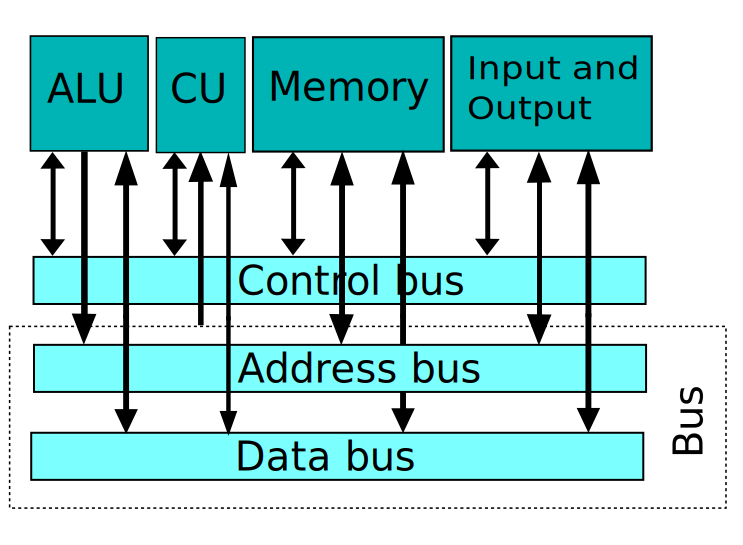
\includegraphics[width=0.5\textwidth]{figures/VNA}
  \end{center}
  \caption{The Von Neumann Architecture. Adapted from \cite{fig-vna}}\label{fig:vna}
\end{figure}

A microinstruction is typically referring to the state of all control signals and is typically generated by the microcode. As it would be extremely inefficient, due to repetition, to only program a computer with individual control signals, the control signals are grouped into microinstructions. The microinstructions are then generated by a net of logic gates or a storage depending on the macro instruction and the current state of the computer.

The pioneering approach of the Von-Neumann-Architecture however was to store the instructions in the same physical memory as the data which simplified the programming process by allowing other programs (compilers, interpreters) to translate from more abstract languages. As instructions and data are stored in the same memory, they must also share the same physical bus. This however leads  to a phenomenon known as the \textit{von Neumann bottleneck} \cite{cit.needed}, where the bus and memory are the limiting factor in the speed of the computer. 

The \textit{von Neumann bottleneck} arises because both the instruction fetch and all data operations must share the same bus and can only occur one after the other, creating a point of congestion. When taking into account that (random access) memory retrieval takes significantly longer than any other operation this bottleneck can be alleviated by introducing a secondary form of memory. Deviating from the Von-Neumann-Architecture the memory module shall be split up into to two modules, a random access memory, storing data and instructions referenced by addresses and the registers, storing a single bus width of data. As well as a number of registers, storing operand data for the alu. The registers function without an address and are directly operated by the control unit.

The modules, in which this architecture is split up to, thus are the ALU, the CU, the memory, the register and the input and output. 

\begin{figure}[H]
  \begin{center}
    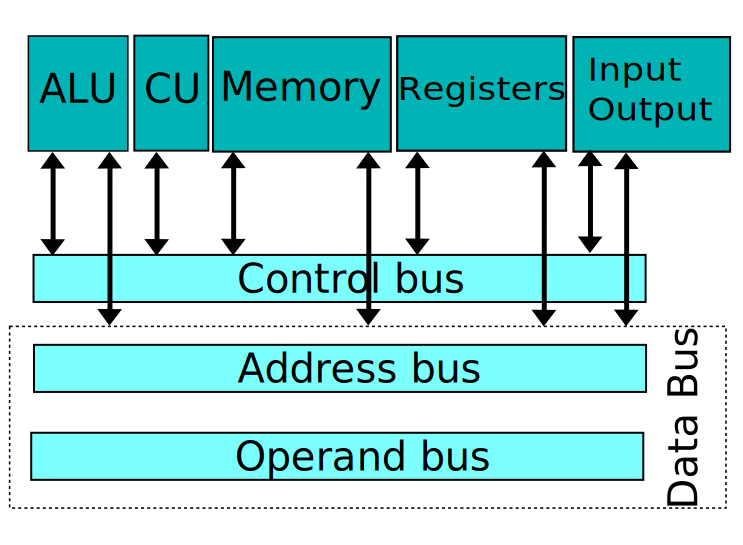
\includegraphics[width=0.5\textwidth]{figures/VNA-Adapted}
  \end{center}
  \caption{The Von Neumann Architecture. Adapted from \cite{fig-vna}}\label{fig:vna-adapted}
\end{figure}

The combined address and data bus is from here on out refered to as the bus.


\iffalse
\begin{figure}[H]
  \begin{center}
  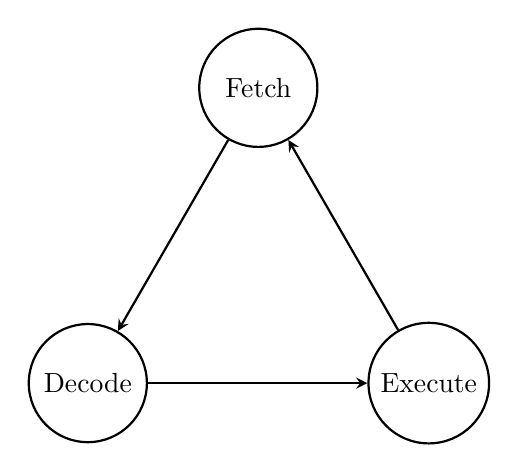
\begin{tikzpicture}[
      node distance=2cm,
      every node/.style={circle, draw, minimum size=1.5cm, align=center},
      ->, >=stealth, thick
  ]

  % Nodes arranged in a circular pattern
  \node (fetch) at (90:2.5cm) {Fetch};
  \node (decode) at (210:2.5cm) {Decode};
  \node (execute) at (330:2.5cm) {Execute};

  % Arrows connecting nodes
  \draw[->] (fetch) -- (decode);
  \draw[->] (decode) -- (execute);
  \draw[->] (execute) -- (fetch);

  \end{tikzpicture}
  \end{center}
  \caption{The fetch-decode-execute cycle \cite{chatgpt}}\label{fig:fde}
\end{figure}
\fi



\subsection{Arithmetic Logic Unit}

\begin{turing-requirement}
  Ability to add two data words.
\end{turing-requirement}

\begin{turing-requirement}
  Generation of at least one status flag (overflow, underflow and/or remainder of divison). 
\end{turing-requirement}

\begin{arch-requirement}
  Ability to take in data from 2 registers.
\end{arch-requirement}

\begin{arch-requirement}
  Ability to output data to the bus. 
\end{arch-requirement}

\begin{arch-requirement}
  Ability to execute all calculations within one timing state.
\end{arch-requirement}

\begin{feat-requirement}
  Ability to subtract two data words.
\end{feat-requirement}

\begin{feat-requirement}
  Ability to multiply two data words.
\end{feat-requirement}

\begin{feat-requirement}
  Ability to divide two data words.
\end{feat-requirement}

\begin{feat-requirement}
  Ability to shift a data word bitwise.
\end{feat-requirement}

\begin{feat-requirement}
  Ability to rotate a data word bitwise.
\end{feat-requirement}

\begin{feat-requirement}
  Must not exert undefined behaviour in case of undefined control signals. 
\end{feat-requirement}

\begin{feat-requirement}
  Must not output unless control signals indicate to do so. 
\end{feat-requirement}

\begin{feat-requirement}
  Ability to AND, OR and XOR two data words.
\end{feat-requirement}

\begin{feat-requirement}
  Ability to perform NOT on a data word.
\end{feat-requirement}


Given those requirements a list of signals going into and out of the module can be compiled. 

\begin{table}[]
\begin{tabular}{ccc}
Type& Name & Purpose \\ \hline
I   & Clock & Timinga \\
O   & Bus     & Data output         \\
I   & Register 1 and 2 & Data input \\
I   & ALU control word & Control \\
O   & Status flag word & Control
\end{tabular}
\caption{}
\label{tab:alu-i/o}
\end{table} 


\subsection{Memory}

\begin{feat-requirement}
Must allow writing to and reading from a memory location
\end{feat-requirement}

\begin{feat-requirement}
Must store, for each memory address, store two data words. 
\end{feat-requirement}

\begin{feat-requirement}
Must retrieve (reword, both retrieve and access) data with an absolute memory address. 
\end{feat-requirement}

\begin{feat-requirement}
Must retrieve data with a relative memory address. 
\end{feat-requirement}

\begin{feat-requirement}
    Must be able to store the program counter and memory address register.
\end{feat-requirement}

\subsection{Registers}

Registers are technically speaking redundant, as the computer already has a form of memory. In practice regs still exist: 
- Regs are in silicon accessible faster than memory. 
- Storage acccess in case of this specific arch is simpler w/o relative addressing etc. 
- ALU needs access to what it calculates, thus registers, unless directly connected to memory, which in practice is not possible (memory seperate silicon from chip). 
Thus registers are considered feature requirements

\begin{feat-requirement}
  Ability to store a data word.
\end{feat-requirement}

\begin{feat-requirement}
  Ability to output a data word.
\end{feat-requirement}

\begin{turing-requirement}
  Ability to load a data word for storage.
\end{turing-requirement}


\subsection{Control Unit}

The Control Unit:
\begin{arch-requirement}
  Must produce the control word from instruction and clock.
\end{arch-requirement}

\begin{turing-requirement}
  Must produce the control word from flags.
\end{turing-requirement}

\begin{feat-requirement}
  Must, given a specific output of the microcode break out of the current instruction. 
\end{feat-requirement}

\begin{feat-requirement}
  Must be reprogrammable for every computer run.
\end{feat-requirement}


% end subsection Control Unit


\input{2-mainpart/architecture/input_output}
